\section{Ergebnisse der Betriebsszenarien}
In dem Kapitel \ref{s:Betriebsszenarien} wurden drei Szenarien für den Vergleich aufgestellt, 
in diesem Abschnitt werden sie ausgewertet und miteinander verglichen. 
Erstens werden die Betriebskosten unter sich verglichen, 
zweitens die benötigten Infrastrukturkosten für jedes Szenario und schließlich 
werden die Szenarien unter Berücksichtigung beider Aspekte betrachtet. 
Die detaillierten Ergebnisse für die Betriebsszenarien sind in Anhang B1.2 zu finden.
%
\subsubsection{Betriebskosten}
Obwohl der Unterschied der Betriebskosten gleichmäßig ist, 
hat unter allen Betriebsszenarien das zweite die höchsten Gesamtbetriebskosten (siehe Abb. \ref{res_betriebsszenarien}). 
Das Erste hat die geringsten Kosten und ist nur etwa 4 \% geringer als das Zweite.
Erkennbar ist auch, dass die Betriebskosten, die durch Batterieantrieb verursacht werden, 
am geringsten unter allen Szenarien sind.
In dem \textbf{zweiten Szenario} entsteht Großteil (57 \%) der Kosten durch wasserstoffbetriebene-Flugzeuge. 
Weitere 38 \% verursacht das SAF.
\textbf{Erstes Szenario} hat den niedrigsten Betriebswert. 
%Die Kosten des ersten Szenarios teilen sich folgend auf. 
Der Betrieb mit SAF verursacht in diesem Szenario die meisten Kosten, nämlich 61 \%.
Etwa ein Drittel der Kosten sind mit dem Betrieb durch Wasserstoff verbunden. Batteriebetriebene 
Flugzeuge haben in diesem Szenario die geringsten verbundenen Betriebskosten (12 \%).
Das \textbf{dritte Szenario} hat 1 \% geringere Kosten als das zweite und somit 
keine signifikante Differenz aufweist. 
Der stärkste Einfluss in diesem Fall geht, ebenso wie im ersten Szenario, 
vom Betrieb mit Wasserstoff aus (48 \%), gefolgt von SAF (44 \%).

\begin{figure}[h]
	\centering
	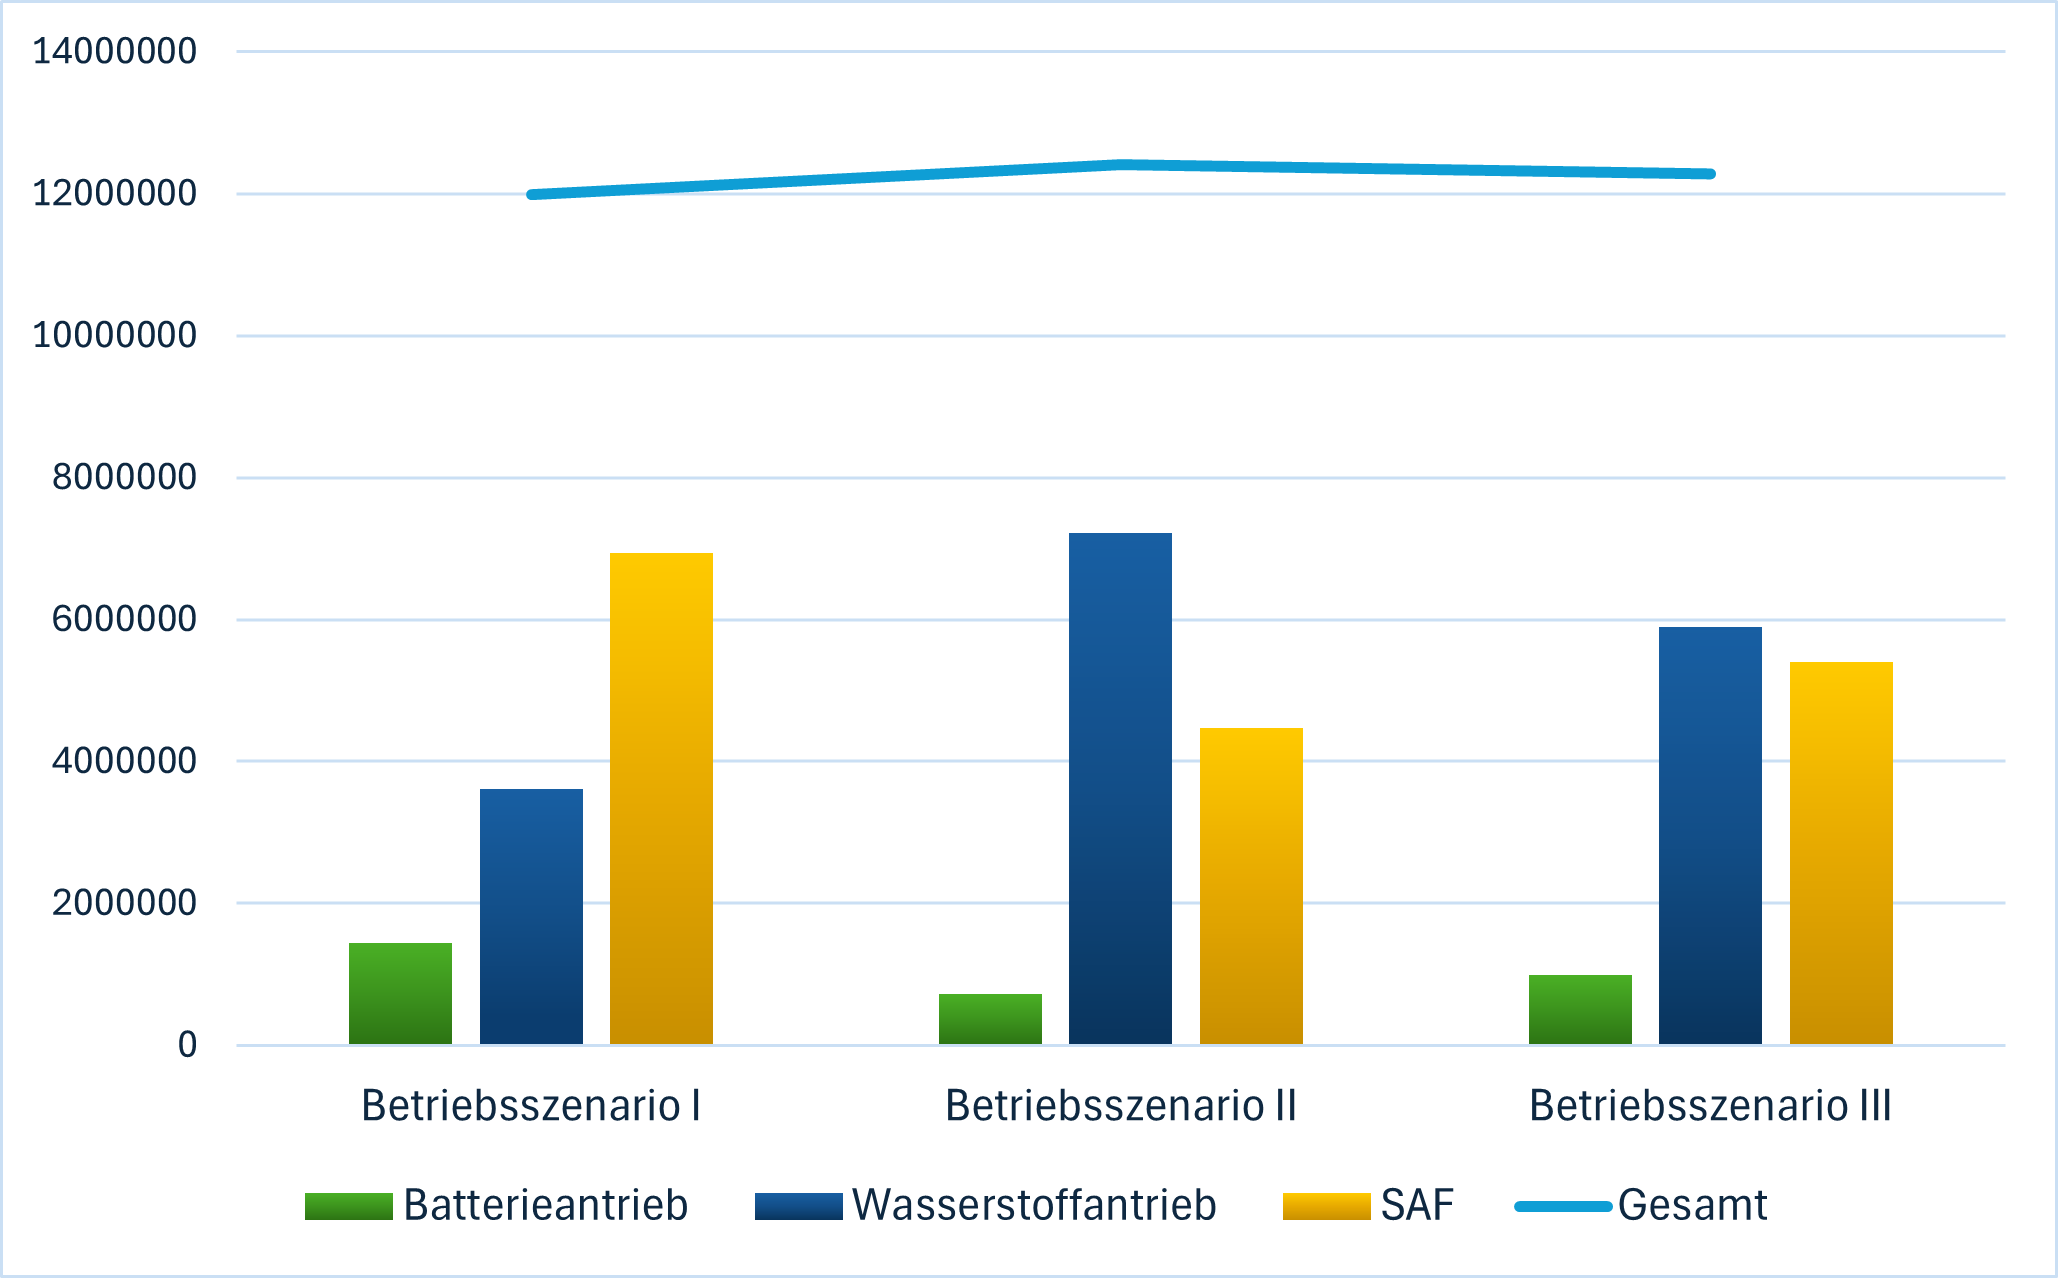
\includegraphics[width=0.8\linewidth]{Bilder/betriebssz_res.png}
	\caption[Betriebskosten in Abhängigkeit von Szenarien mit Gesamtkostentrend]{Betriebskosten in Abhängigkeit von Szenarien mit Gesamtkostentrend}
	\label{res_betriebsszenarien}
\end{figure}

\subsubsection{Infrastrukturkosten}
In der Tabelle \ref{Infrastrukturwerte_res} sind die benötigten 
Infrastrukturanschaffungswerte für jedes Szenario zusammengefasst. 
Die Werte wurden anhand der vorgeschlagenen Methodik ermittelt.\\
%
\begin{table}[h]
	\begin{center}
    \caption{Infrastrukturwerte für Wasser- und Batterieantrieb für alle Szenarien}
	\label{Infrastrukturwerte_res}
	\begin{tabular}{|l|c|c|c|}
		\hline
		 & \textbf{Szenario I}& \textbf{Szenario II}& \textbf{Szenario III} \\ \hline
		Anzahl Ladestationen $n_{BSS}$ & 20 & 10& 14\\ \hline
		Anzahl Batterien $n_{Bat}$ & 101 & 51& 70 \\ \hline
		Anzahl Betankungswagen $n_{BW}$ & 4 & 7 & 5\\ \hline
		Anzahl Pumpen $n_{kP}$  & 5 & 8 & 6\\ \hline
	\end{tabular}
    \end{center}
\end{table}
%
Nennenswert ist, dass in der Berechnung von allen Betriebsszenarien erstmal nur einmalige Infrastrukturausgaben 
ohne jährliche Abschreibungen ausgerechnet sind (siehe Abb. \ref{res_betriebsszenarien}). 
Das erste Szenario hat die geringsten Ausgaben, wobei das zweite Szenario die höchsten (27 \% höher als das Erste) hat.
Die Gesamtkosten für das zweite Szenario liegen bei über 35 Tausend Euro. %Die konkreten Ergebnisszahlen sind in der Anhang XX zu finden.
Im ersten Szenario zeigt sich, dass die Preisaufteilung für Batterie- und Wasserstoffinfrastruktur nahezu gleiche Anteile aufweist.
In den anderen Szenarien führen die Kosten für die Wasserstoffinfrastruktur.\\
\begin{figure}[h]
	\centering
	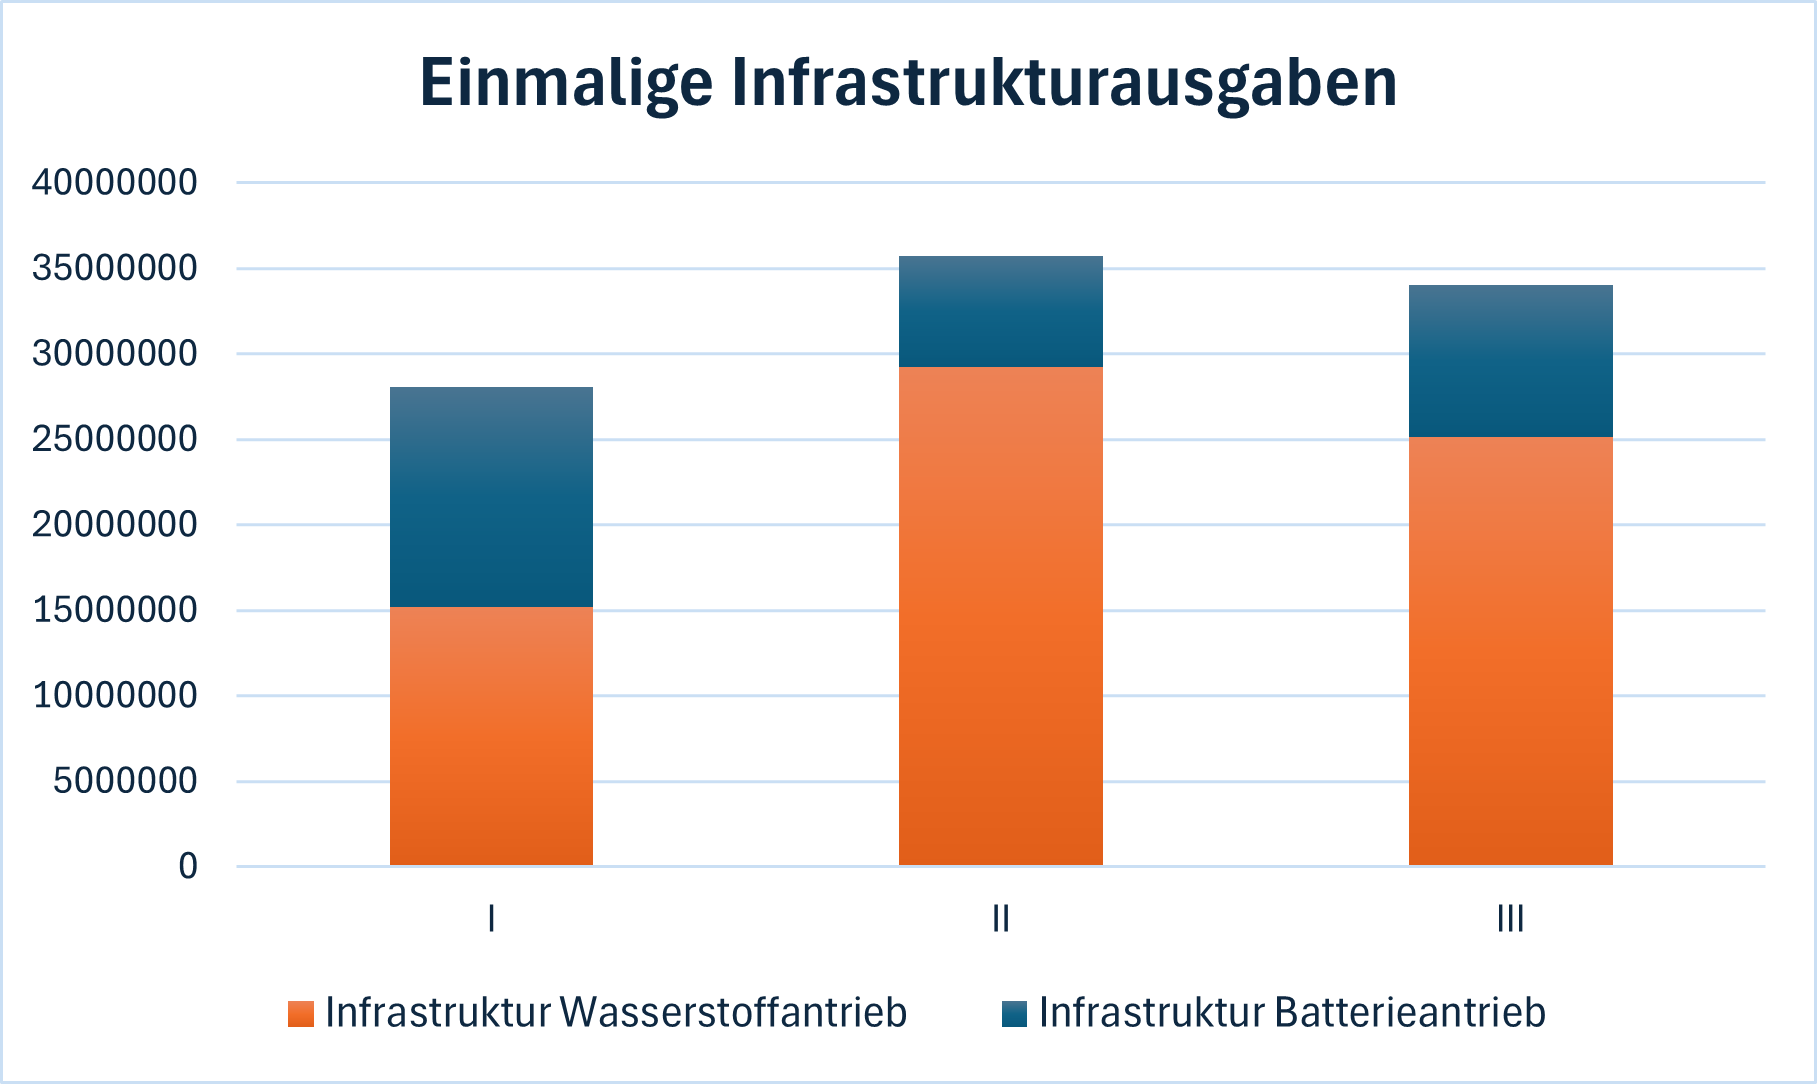
\includegraphics[width=0.8\linewidth]{Bilder/Infr_Szenarien.png}
	\caption[Vergleich der einmaligen Infrastrukturausgaben zwischen den Betriebsszenarien]{Vergleich der einmaligen Infrastrukturausgaben zwischen den Betriebsszenarien. Die schwarzen Linien
	zeichnen minimale und maximale Reduzierungen basierend auf den aufgestellten Szenarien}
	\label{res_infr_betriebsszenarien}
\end{figure}
%
Wird die lineare jährliche Abschreibung mitbetrachtet, sehen die Ergebnisse anders aus. 
Diese Erkenntnisse stützen die dritte Hypothese.
Die erheblichsten Kosten entstehen im ersten Szenario, 
wobei dieses Szenario bei einmaligen Ausgaben das beste Ergebnis erzeugt.
Die geringsten jährlichen Abschreibungskosten würde das zweite Szenario liefern, 
obwohl es die höchsten einmaligen Ausgaben hat. 
Demnach kann eine ungünstige Wahl der Abschreibungsverteilung die anfangs günstigeren Ausgaben 
im Vergleich zu anderen Szenarien steigen lassen, womit die dritte Hypothese bewiesen wurde.\\
%
\begin{figure}[h]
	\centering
	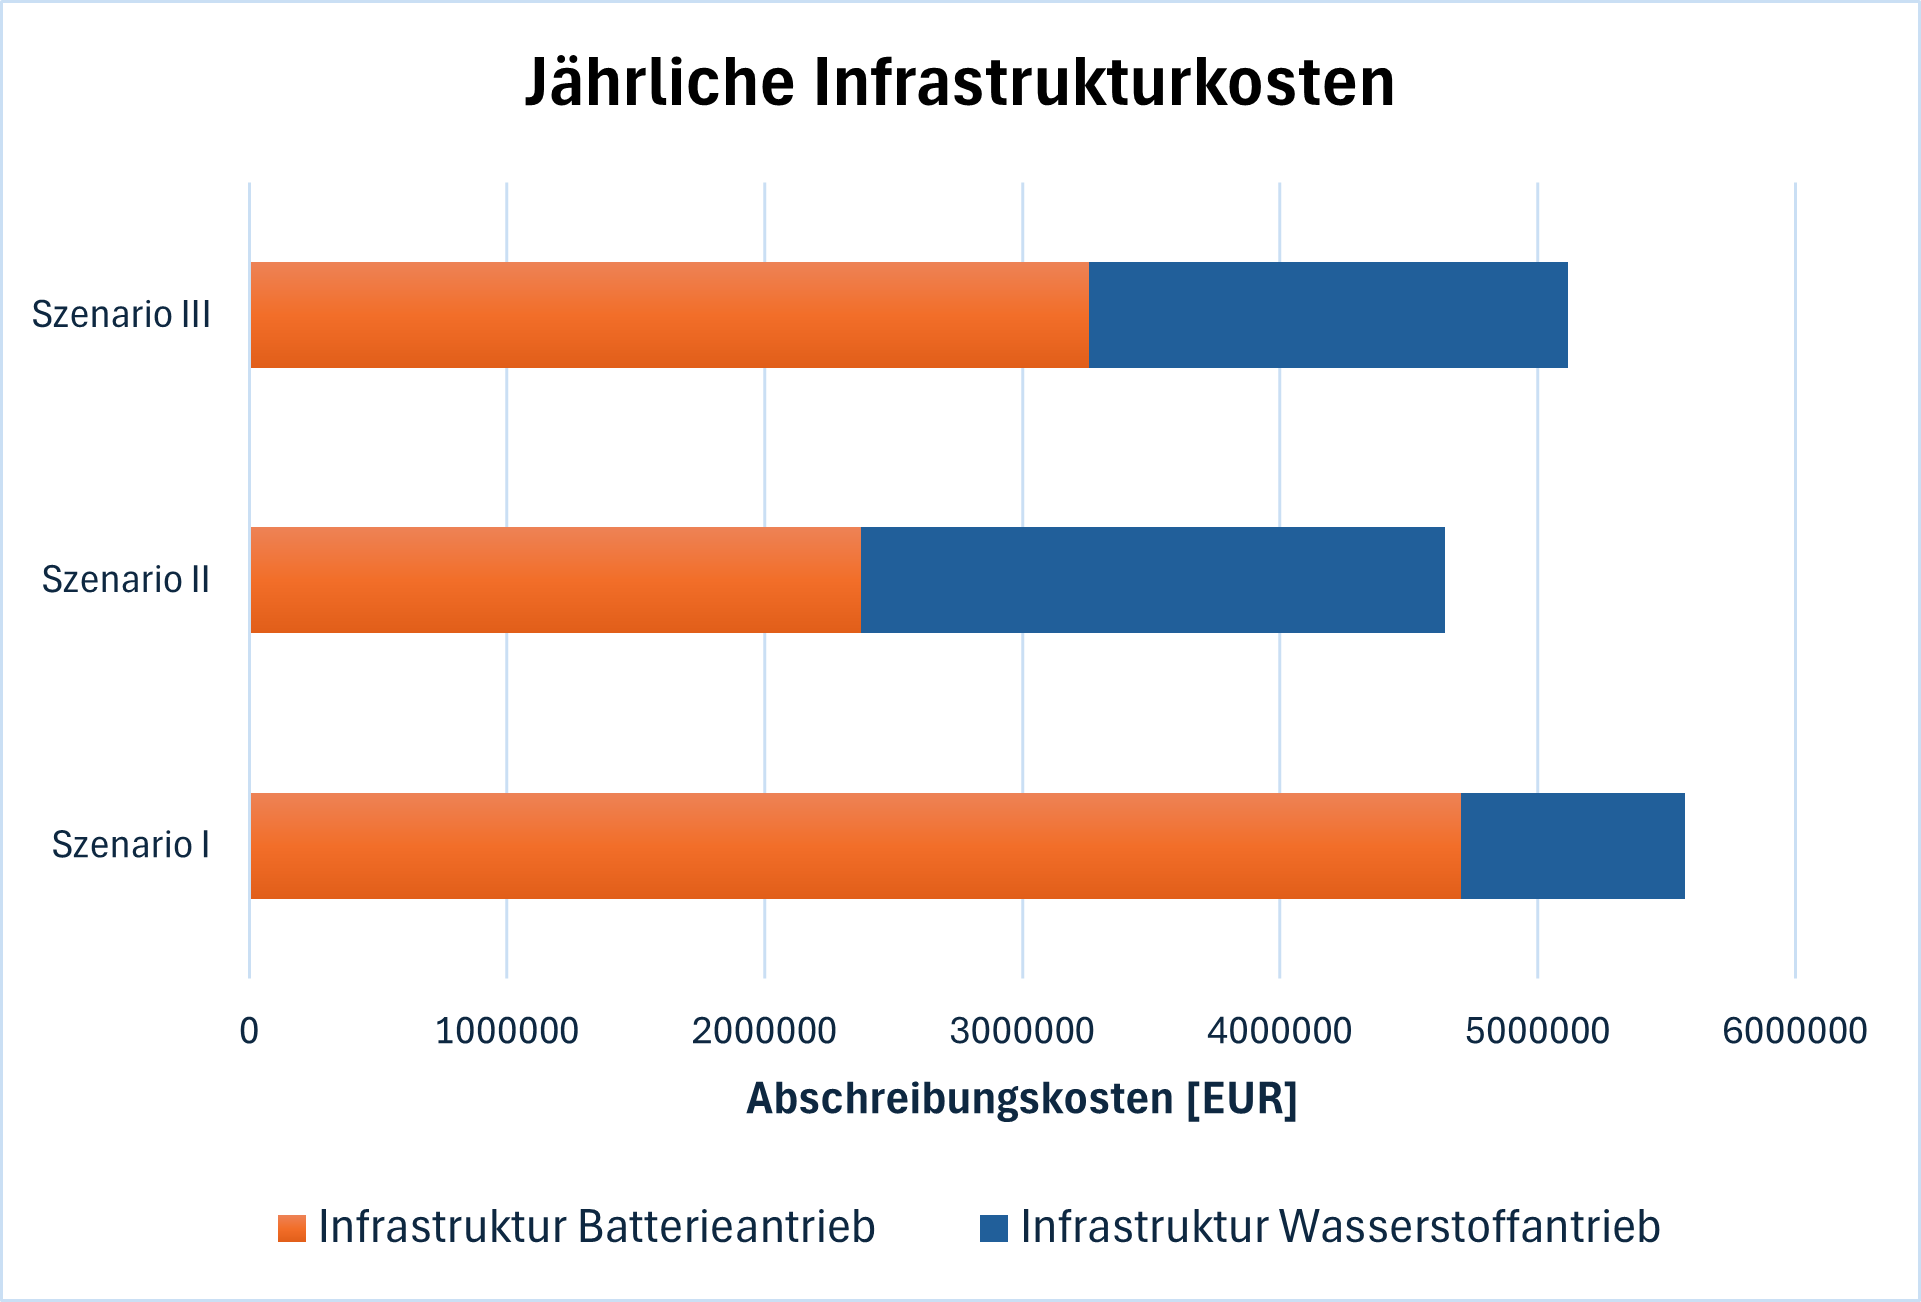
\includegraphics[width=0.8\linewidth]{Bilder/infr_abschreibung.png}
	\caption[Vergleich der jährlichen Infrastrukturausgaben zwischen den Betriebsszenarien]{Vergleich der jährlichen Infrastrukturausgaben zwischen den Betriebsszenarien}
	\label{res_betriebsszenarien}
\end{figure}

